% -*- TeX -*- -*- DE -*-

\chapter{PatchCore \cite{patchcore}}\label{ch:PatchCore}
\section{Einleitung}\label{sec:EinleitungPatchCore}
Die Methode \textbf{PatchCore} wurde erstmals am 15. Juni 2021 in Zusammenarbeit der Universität Tübingen und Amazon AWS im Paper \glqq Towards Total \ 
Recall in Industrial Anomaly Detection\grqq{} veröffentlicht. \ 
In seiner zweiten Fassung vom 5. Mai 2022 wurde das Paper bei der Konferenz CVPR 2022 (Computer Vision and Pattern Recognition) akzeptiert und mit \ 
über 290 Zitierungen eines der populärsten Paper im Bereich der Unüberwachten Anomaliedetektion.\\
Die Grundlage dieses Ansatzes sind wiederum \glqq Einbettungen\grqq{} (Embeddings) von Merkmalen (Features), \ 
die aus den Eingabebildern mithilfe eines auf \glqq ImageNet\grqq{} vortrainiertem \glqq Convolutional Neural Network (CNN)\grqq{} erzeugt werden.\
Damit ähnelt sich die Methode PatchCore sowohl SPADE\ref{sec:SPADE}, also auch PaDiM\ref{sec:PaDiM} und greift die in \ref{subsec:ResNetsAsFeatureExtractor} \
beschriebene Vorgehensweise auf.\
Wie wir später sehen werden, unterscheidet sich der Einbettungsprozess jedoch recht deutlich von den bisherigen Methoden.\
% Wie in einigen vorangegangenen Veröffentlichungen im Bereich der Unüberwachten Anomaliedetektion, werden auch hier die Features in \glqq Patches\grqq{} \ 
% unterteilt, um die Lokalität der Anomalien zu erhalten. Diese werden folgend als \textbf{\glqq Patch Features\grqq{}} bezeichnet.\
Weiter wird die eigentliche Anomaliedetektion, wie bereits bei der Methode SPADE mithilfe einer Nächsten Nachbar Suche \ 
(Nearest Neighbor Search; NN) in einer \glqq Memory-Bank \grqq{} durchgeführt.\
Die wesentliche Weitereentwicklung gegenüber SPADE liegt vor allem in der Methode, wie die Memory-Bank aufgebaut wird. Durch die Auswahl möglichst representativer \
Elemente in der Memory Bank, kann die Anzahl der Elemente in der deutlich reduziert werden, was einer Reduzierung der Laufzeit bedeutet.\\
Auch gut 2 Jahre nach Veröffentlichung ist die PatchCore Methode insbesondere auf dem MVTecAD-Datensatz\ref{sec:DatensatzMVTecAD} mit einer Genauigkeit (Auccuracy) \ 
von maximal \num{99,6}\% (\glqq PatchCore Ensemble\grqq{}) absolut konkurrenzfähig und wird in vielen Veröffentlichungen als \glqq State-of-the-Art\grqq{} Methode verwendet.\\
Im Laufe dieses Kapitels soll zunächst die Funktionsweise der Methode PatchCore erläutert werden. Anschließend evaluieren wir die Originalmethode im Hinblick auf Laufzeit und Genauigkeit. \
Im sich dann anschließenden Teil werden zahlreiche Modifikationen besprochen, die versuchen, die Laufzeit auf zu Reduzieren und dabei möglichst viel der Genauigkeit zu erhalten.\

% Zunächst wollen wir die grundsätzliche Funktionsweise der Methode PatchCore erläutern. Anschließend bewerten wir die Methode im Hinblick auf Laufzeit und Genauigkeit. \
% Anschließend werden zahlreiche Adaptionen der Methode vorgestellt, die im Sinne des Ziels dieser Arbeit die Laufzeit der Methode reduzieren und dabei die Genauigkeit möglichst wenig beeinträchtigen sollen.\
\section{Funktionsweise}
\label{sec:Funktionsweise}
unächst kann zwischen zwei Phasen unterschieden werden: Der Trainingsphase und der Testphase.\
In der Trainingsphase werden die \glqq (locally aware) \textbf{Patch Features}\grqq{} aus den Trainingsbildern (\glqq Nominal Samples\grqq{}) extrahiert. \ 
Hierzu wird ein \glqq Pretrained Encoder\grqq{} verwendet, analog zu \ref{subsec:ResNetsAsFeatureExtractor}.\
Anschließend findet eine Unterabtastung bzw. eine Auswahl der Patch Features statt, die in der \glqq Memory Bank\grqq{} gespeichert werden. \ 
Dieser Vorgang wird als \glqq Coreset Subsampling\grqq{} bezeichnet.Ist diese Memory Bank erzeugt, ist die Methode initialisiert und das Training abgeschlossen.\ 
In der Testphase werden die Patch Features auf die gleiche Weise aus den \glqq Test Samples\grqq{} extrahiert, wie in der Trainingsphase. Jedes dieser Patch Features wird nun mit den Patch Features in der Memory Bank verglichen.\ 
Dies geschieht mit einer \glqq Nearest Neighbor Search\grqq{} (NN). Aus den Distanzen zum Nächsten Nachbarn kann dann, wie in \ref{sec:PaDiM} eine räumlich aufgelöste anomaliekarte erzeugt werden.\ 
Auf Grundlage dieser Anomaliekarte geschieht dann die Instanzklassifizierung als nominal oder anomal. Nachfolgende Abbildung \ref{fig:PatchCore}, die aus der Veröffentlichung übernommen wurde, zeigt \ 
die Funktionsweise der Methode PatchCore.\
\begin{figure}[h]
    \centering
    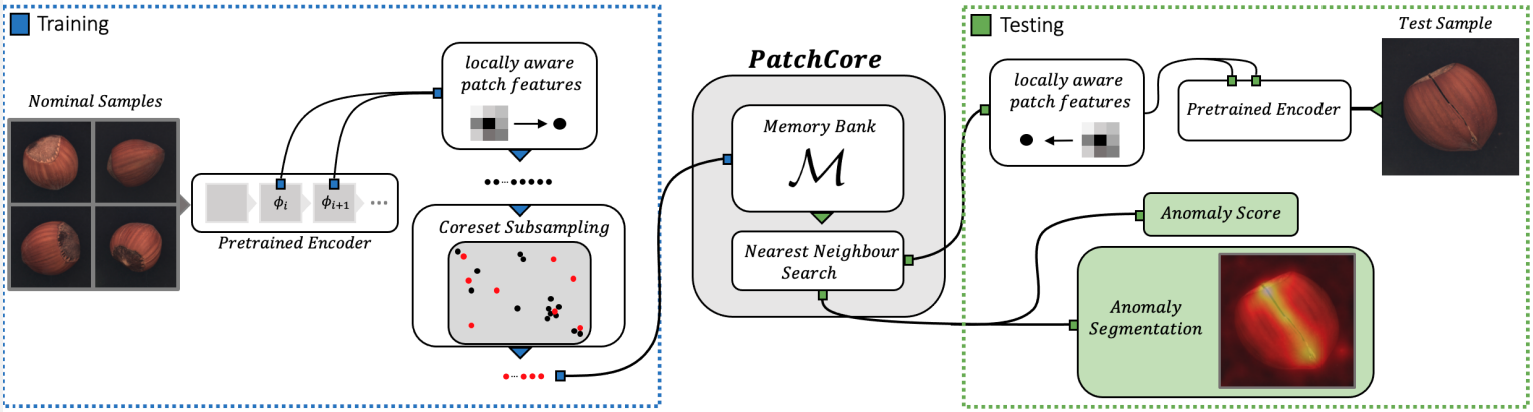
\includegraphics[width=0.95\textwidth]{bilder/patchcore.png}
    \caption{PatchCore}
    \label{fig:PatchCore}
\end{figure}
\subsection{Erzeugen der Patch Features}\label{subsec:ErzeugenDerPatchFeatures}
Zunächst werden einige Notationen definiert, die im Folgenden verwendet werden. Es wird sich dabei auf die Notationen aus der Veröffentlichung bezogen.\
So wird die Menge aller Trainingsbilder als $\mathcal{X}_{train}$ bezeichnet. Die Menge aller Testbilder als $\mathcal{X}_{test}$.\
Für den Trainingsdatensatz gilt im Sinne der Unüberwachtheit, dass es sich um ausschließlich nominale Samples handelt. Im Testdatensatz können sowohl nominale als auch anomale Samples enthalten sein.\
% Werden nominale Samples mit $0$
Bezeichnen wir die wahre Klassenzugehörigkeit eines Bildes $x$ als $y_{x}$, so kann diese entweder $0$ (nominal) oder $1$ (anomal) sein. Für den Trainingsdatensatz gilt dann:\
$\forall x \in \mathcal{X}_{train}: y_{x} = 0$ und für den Testdatensatz $\forall x \in \mathcal{X}_{test}: y_{x} \in \{0,1\}$.\\
Den bereits in \ref{sec:SPADE} und \ref{sec:PaDiM} angetroffenen \glqq Pretrained Encoder\grqq{} wird als $\phi$ bezeichnet.\
Es wird dabei, wie bereits gesehen, nicht der Ausgang dieses Netzwerkes benutzt, sondern die Feature Maps aus einer bestimmten Schicht $j$ des Netzwerkes. \
Im Falle von ResNets, die auch in dieser Veröffentlichung hauptsächlich verwendet werden, ist $j\in \{1,2,3,4\}$.\ 
$j$ wird folgend auch als \glqq Hierarchielevel\grqq{} bezeichnet und spielt eine wichige Rolle.\
$\phi_{i,j} = \phi_{j}(x_{i})$ bezeichnet die Feature Map des Bildes $x_{i}\in \mathcal{X}$ aus dem Hierarchielevel $j$.\
Wie bereits in \ref{subsec:SPADEResults} diskutiert, ist eine sinnvolle Auswahl der Hierarchielevel eine wichtige Voraussetzung für gute Ergebnisse.\
Auch die Autoren von PatchCore weisen auf diese Problemstellung hin. Man könne, wie bei SPADE, die letzte Ebene in der Merkmalshierarchie des Netzes verwenden. \
Dies bringe aber die folgenden zwei Probleme mit sich. Erstens gehe dabei mehr lokalisierte nominale Informationen verloren. Das sei während der Trainingsphase kritisch, \
weil die Arten von Anomalien, die zum Testzeitpunkt auftreten, nicht im Voraus bekannt seien und die möglichst vollständige Erfassung des Normals notwendig sei.\
Zweitens seien die sehr tiefen und abstrakten Merkmale in den vortrainierten ImageNet-Netzwerken auf die Aufgabe der Klassifizierung natürlicher Bilder ausgerichtet, \ 
welche nur wenig direkte Überschneidungen mit der hier vorliegenden Aufgabe der industriellen aufweise. \
Es wird deshalb vorgeschlagen, Merkmale aus den mittleren Hierarchieleveles zu verwenden. Das entspricht bei ResNets $j\in \{2,3\}$.\
Wie in \ref{fig:ResNetPyramid} zu erkennen, handelt es sich bei $\phi_{i,j}$ um einen dreidimensionalen Tensor: $\phi_{i,j}\in \mathbb{R}^{c^{*}\times h^{*}\times w^{*}}$\
mit $c^{*}$ als Tiefe der Feature Maps, $h^{*}$ als Höhe und $w^{*}$ als Breite. \
$\phi_{i,j}(h,w)\in\mathbb{R}^{c^{*}}$ bezeichnet dann den zur Position $h\in\{1,...,h^{*}\}$ und $w\in\{1,...,w^{*}\}$ gehörenden Vektor der Länge $c^{*}$.\
Unter der Annahmen, dass die Größe des Feldes im Originalbild $x_{i}$, das Einfluss auf ein $\phi_{i,j}(h,w)$ nimmt (\glqq Receptive Field\grqq{}), \
ausreichend groß ist, um einen ausreichenden räumlichen Kontext zu erfassen, eignet sich dieser Vektor als \glqq Patch Feature\grqq{} für eine gegenüber \ 
räumlichen Variationen robuste Anomaliedetektion.\\
Um diese wünschenswerte Annahme zu erfüllen, wird eine Aggregation der lokal umliegenden Regionen (\glqq local Neighborhood Aggregation\grqq{}) durchgeführt, das nachfolgend \
vorgestellt wird und die Größe des Receptive Fields steuert.\\
Dafür wird die oben eingeführte Notation für $\phi_{i,j}(h,w)$ um eine ungerade Feldgröße (\glqq patchsize\grqq{}) $p$ erweitert, die die benachbarten Feauture Vektoren \
mit einbezieht. Zunächst wird diese Nachbarschaft wie folgt definiert:\
$$
\mathcal{N}_{p}^{(h,w)} = \left\{(a,b)| a \in \left[h-\left\lfloor \frac{p}{2}\right\rfloor,...,h+\left\lfloor \frac{p}{2} \right\rfloor\right], b \in \left[w-\left\lfloor \frac{p}{2}\right\rfloor,...,w+\left\lfloor \frac{p}{2}\right\rfloor\right]\right\}
$$ 
Damit ergeben sich schließlich ein \glqq Patch Feature\grqq{} zu\
$$
\phi_{i,j}\Big(\mathcal{N}_{p}^{(h,w)}\Big) = f_{agg}\Big(\{\phi_{i,j}(a,b)| (a,b) \in \mathcal{N}_{p}^{(h,w)}\}\Big),
$$
wobei $f_{agg}$ eine Aggregationsfunktion ist. Die Aggregationsfunktionsfunktion, die in der PatchCore Methode verwendet wird, ist ein adptives \glqq Average Pooling\grqq{}, \
in einer Dimension, die unabhängig von der Länge der Eingangsfeature, immer eine feste Länge $d$ ausgibt.\\
Da diese Operation für alle Paare von $(h,w)$ mit $h\in\{1,...,h^{*}\}$ und $w\in\{1,...,w^{*}\}$ durchgeführt wird, wird die Auflösung der Feature Map erhalten.
Für einen gesamten Feature Map Tensor ergibt sich dementsprechend:\
$$
\mathcal{P}_{s,p}\left(\phi_{i,j}\right) = \left\{\phi_{i,j}\Big(\mathcal{N}_{p}^{(h,w)}\Big)| h\in\{1,...,h^{*}\}, w\in\{1,...,w^{*}\}\right\}
$$
Wie bereits erwähnt, geschieht diese Operation für verschiedene Hierarchielevel $j$.\ Weil die Auflösung der Feature Maps mit steigendem Hierarchielevel abnimmt, \
wird $\mathcal{P}_{s,p}\left(\phi_{i,j+1}\right)$ berechnet und anschließend auf die Auflösung von $\mathcal{P}_{s,p}\left(\phi_{i,j}\right)$ bilinear interpoliert.\ 
Jedes Element wird dann mit dem korrespondieren Element, also dem Element an der gleichen Stelle, aggregiert.\
Würde auf eine Auswahl der Patch Feature, wie im folgenden Abschnitt erläutert, verzichtet, würde sich folgende Memory-Bank ergeben:
$$
\mathcal{M} = \bigcup_{x_i\in\mathcal{X}_{train}}\mathcal{P}_{s,p}\left(\phi_{i,j}\right)
$$
\subsection{Coreset Subsampling}\label{subsec:CoresetSubsampling}
Insbesondere, wenn $\mathcal{X}_{train}$ eine große Kardinalität hat, also viele Bilder hat, wird die Memory-Bank $\mathcal{M}$ sehr groß. Wie bereits in \ref{sec:SPADE} festgestellt \
ist diese Kardinalität besonders laufzeitkritisch, weil die Nächste Nachbar Suche in der Memory-Bank mit einer Komplexität von $\mathcal{O}(n)$ berechnet wird. \ 
Wie bereits in \ref{sec:PaDiM} zu sehen, ist ein \glqq patchbasierter\grqq{} Vergleich zwischen allen Elementen in $\mathcal{M}$ und allen Elemnten in $\mathcal{P}_{s,p}\left(\phi_{i,j}\right)$ \
ein notwediger Schritt, nicht nur um die Anomaliekarte zu erstellen, die in dieser Arbeit ohnehin von keinem großen Interesse ist, sondern auch um eine robuste und \ 
präzise Instanzklassifizierung durchzuführen. Für die Laufzeitoptimierung ist es also wünschenswert, die Kardinalität der Memory-Bank zu reduzieren.\\
Auf der anderen Seite müssen die Elemente in $\mathcal{M}$ möglichst gut nominale Eigenschaften abbilden, um eine gute Anomaliedetektion zu ermöglichen.\
Wie in der Veröffentlichung gezeigt wird, (§4.4.2 - Importance of Coreset Subsampling) führt der naive Ansatz, zufällig Elemente aus $\mathcal{M}$ auszuwählen, \
nicht zu zufriedenstellenden Ergebnissen.\\
Das von PatchCore zugrundeliegenden Konzept setzt genau hier an. Es soll eine Teilmenge $\mathcal{S}\subset \mathcal{A}$ gefunden werden, bei der die Problemlösung \
über $\mathcal{A}$ am ehesten und vor allem schneller durch die über $\mathcal{S}$ berechnete Lösung approximiert werden kann. Dabei ist die Methode, \
die zu einer solchen Teilmenge führt, problemspezifisch. Im Falle von PatchCore wird eine Berechnung von Nächsten Nachbarn durchgeführt, \
weswegen gemäß \cite{sener2018active} ein \glqq MiniMax-Funktion\grqq{} sich anbietet, um eine annähernd ähnliche Abdeckung der $\mathcal{M}$ mit $\mathcal{M_{C}}$ zu erreichen.\
Dies kann wie folgt gelöst werden:\
$$
\mathcal{M_{C}^{*}} = \underset{\mathcal{M}_{C}\subset\mathcal{M}}{\arg\min}\underset{m\in\mathcal{M}}{\max}\underset{n\in\mathcal{M_{C}}}{\min}\left\|m-n\right\|_{2}
$$
Die exakte Berechnung von $\mathcal{M_{C}^{*}}$ ist NP-schwer, also nicht in polynomieller Zeit berechenbar.\
Es handelt sich zwar um einen Prozess, der nicht während der Inferenz durchgeführt werden muss, sondern einmalig während der Trainingsphase, \
aber es muss dennoch mit iterativen, approximierenden Verfahren gearbeitet werden.\\
Aus \cite{sener2018active} wird ein \glqq Greedy Algorithmus\grqq{} übernommen, der iterativ Elemente aus $\mathcal{M}$ auswählt, die die größte Distanz zu allen bereits ausgewählten Elementen haben.\
Um die Laufzeit des Subsamplings weiter zu reduzieren, wird das \glqq Johnson-Lindenstrauss Lemma\grqq{}\cite{johnsonlindenstrauss} verwendet, um die Dimensionalität der Elemente $m\in\mathcal{M}$ \ 
durch zufällige lineare Projektion $\psi: \mathbb{R}^{d} \rightarrow \mathbb{R}^{d^{*}}$ mit $d^{*}<d$ zu reduzieren. Anschaulich kann dies durch eine Punktwolke erklärt werden, die aus zufälligen Blickwinkeln betrachtet wird, wodurch die 3-D-Struktur als 2-D Struktur\
angenähert wird. (TODO --> Algorithmus?)\\
\subsection{Bestimmen des Anomaliegrades}\label{subsec:BestimmenDesAnomaliegradesPatchcore}
Wie bereits in der Einleitung zu diesem Katpitel erwähnt, ist die Grundlage der Bestimmung des Anomaliegrades die Distanz zu den Nächsten Nachbarn in der Memory-Bank.\ 
Das gilt sowohl für die Anomaliekarte bzw. die Segmentierung, als auch für die Instanzklassifizierung. \
Zunächst muss während der Inferenz aus einem Testbild $x_{i}\in\mathcal{X}_{test}$ die Patch Features extrahiert werden. Dies geschieht auf die gleiche Weise, wie in der Trainingsphase:\
$$
\mathcal{P}\left(x_{i}\right)= \mathcal{P}_{p}\left(\phi_{j}\left(x_{i}\right)\right)
$$
Diese Menge $\mathcal{P}\left(x_{i}\right)$ enthält nun die Patch Features $m^{test}$ des Testbildes $x_{i}$. Nun gilt es zu jedem Patch Feature in $\mathcal{P}\left(x_{i}\right)$ \
den Nächsten Nachbarn in der Memory Bank $\mathcal{M}$ zu finden:\
$$
m^{*} = \underset{m\in\mathcal{M}}{\arg\min}\left\|m-m^{test}\right\|_{2}, \forall m^{test}\in\mathcal{P}\left(x_{i}\right)
$$
Es gilt zu beachten, dass jedes $m^{test}$ zu einer Position $(h,w)$ im Bild $x_{i}$ gehört.\
So kann eine räumlich aufgelöste Anomaliekarte $M$ erzeugt werden, die die Distanz zu den Nächsten Nachbarn in der Memory-Bank enthält:
$$
% M = \left\{m^{*}(h,w)| m^{*} = \underset{m\in\mathcal{M}}{\arg\min}\left\|m-m^{test}\right\|_{2}, \forall m^{test}\in\mathcal{P}\left(x_{i}\right)\right\}
M = \Big(\left\|m^{*}_{h,w}-m^{test}_{h,w}\right\|_{2}\Big)_{h,w},\forall \left(h,w\right)\in\{1,...,h^{*}\}\times\{1,...,w^{*}\} % m^{test}_{h,w}\in\mathcal{P}\left(x_{i}\right)
$$
Diese Anomaliekarte $M$ kann schließlich mittels bilinearer Interpolation und einer anschließenden Glättung auf die Auflösung des Originalbildes $x_{i}$ gebracht werden, wodurch eine \
pixelweise Klassifikationskarte möglich wird. Weil dies in dieser Arbeit nicht von Interesse ist, wird darauf nicht weiter eingegangen.\\
Die Instanzklassifizierung könnte nun analog zu PaDiM (\ref{subsec:PaDiMFunktionsweise}) durch Maximalwerbildung durchgeführt werden.\
Die Autoren von PatchCore gehen ähnlich vor, fügen jedoch noch einen Gewichtungsschritt hinzu.\
Zunächst wird ganz analog vorgegangen und die maximale Distanz zu den Nächsten Nachbarn herangezogen, was nichts anderes als der Maximalwert der Anomaliekarte $M$ ist.\
$$
m^{test,*}, m^{\star}=\underset{m^{test}\in\mathcal{P}(x_{i})}{\arg\max}\underset{m\in\mathcal{M}}{\arg\min}\left\|m-m^{test}\right\|_{2}
$$
$$
s^{*}=\left\|m^{test,*}-m^{\star}\right\|_{2}=\max\{M\}
$$
Die Gewichtung schließt die nächsten $b$ Patch Features in $M$ zu $m^{\star}$ mit ein. Diese Menge notieren wir als $\mathcal{N}_{b}\left(m^{\star}\right)$.\
Der Gedanke hinter dieser Gewichtung ist, den Anomaliegrad $s$ dann zu erhöhen, wenn die Feature Patches in $\mathcal{N}_{b}\left(m^{\star}\right)$ selbst \
weit entfernt vom Anomaliekandidaten Patch Feature $m^{\star}$ sind und es sich somit ohnehin um seltene nominale Patch Features handelt. \
Der finale, für die Instanzklassifiziergung entscheidende Anomaliegrad $s$ ergibt sich dann zu:\
$$
s = \left(1-\frac{e^{\left\|m^{\star}-m^{test,*}\right\|_{2}}}{\sum\nolimits_{m\in\mathcal{N}_{b}\left(m^{\star}\right)}e^{\left\|m-m^{test,*}\right\|_{2}}}\right) \cdot s^{*}
$$
Durch diese Gewichtung wird die Instanzklassifizierung robuster und erhöht die Instanzklassifiziergungsgenauigkeit, wodurch es eine weitere Weitereentwicklung gegenüber PaDiM darstellt.\
\section{Ergebnisse und Diskussion der Originalmethode}\label{sec:ErgebnisseUndDiskussionDerOriginalmethode}
In diesem Abschnitt werden die Ergebnisse der Originalmethode PatchCore vorgestellt und diskutiert.\
Dies soll vor allem im Hinblick auf die Eignung für eine Implementierung auf einem ressourcenbeschränkten Gerät, nämlich einem RaspberryPi 4B (\ref{sec:RaspberryPi4B}) geschehen.\
Es wird sich dabei auf den hier verwendeten Datensatz MVTecAD (\ref{sec:DatensatzMVTecAD}) bezogen. Weitere Datensätze, die in der Veröffentlichung verwendet wurden, \
werden mit dem Verweis auf die Veröffentlichung nicht weiter betrachtet. Die zur Evaluation herangezogene Metrik ist AUROC (\ref{sec:AUROC}).\\
Wie bereits in der Einleitung erwähnt, ist die Methode PatchCore grundsätzlich in der Lage, sehr hohe Instanzklassifiziergungsgenauigkeiten zu erreichen, die auch zwei Jahre nach \
Veröffentlichung noch zu den besten gehören. Erreicht wird dies teilweise durch ein Ensemble von verschiendenen Feature Extraktoren bzw. Backbones und höhere Auflösungen.\
So wird ein \glqq DenseNet 201\grqq{}\cite{densenet}, ein \glqq ResNext 101\grqq{}\cite{resnext} und ein bereits bekanntes Wide ResNet mit 101 Schichten\cite{wideresnet} verwendet. \
Steht eine GPU zur Verfügung, welche, wie in \ref{tab:model-runtimes} zu sehen, die Laufzeit von CNNs deutlich reduziert, können selbst mit einer solchen Konfiguration, bestehend aus \
vielen Backbones, einigermaßen schnelle Inferenzzeiten erreicht werden.\
Da die Zielsetzung dieser Arbeit jedoch die Implementierung auf einem RaspberryPi 4B ist und bereits gezeigt wurde, dass das Ausführen von CNNs auf einem solchen Gerät \
äußerst laufzeitkritisch ist, ist eine solche Konfiguration im Kontext dieser Arbeit nicht sinnvoll.\
Beschränken wir uns auf Konfigurationen, mit nur einem Backbone und auf die Auflösung von $256\times 256$ Pixeln, so erreicht PatchCore mit einem Wide ResNet-50 Backbone eine \
Instanzklassifiziergungsgenauigkeit (AUROC) von \num{99,1} mit einer Reduktion der Memory Bank auf \num{25}\%. Wird die Größe der Memory Bank auf \num{1}\% reduziert, \
verschlechtert sich der AUROC nur leicht auf \num{99,0}\%. Wie im Laufe dieses Kapitels noch zu sehen sein wird, ist die Reduzierung der Kardinalität der Memory Bank \
ein wichtiger Schritt, um die Laufzeit zu reduzieren. Die hier angewandte Methode des Coreset Subsamplings ist also ein wichtiger Bestandteil und eine Errungenschaft \ 
der Methode PatchCore.\\
Neben dem Erzeugen der Patch Feature ist die Nächste Nachbar Suche in der Memory Bank besonder laufzeitkritisch. In der Veröffentlichung lediglich eine kleine Randnotiz im Anhang, \
ist diese Suche mit \glqq FAISS\grqq{} (TODO --> ref und cite) implementiert. FAISS ist eine Bibliothek, entwickelt von Facebook's AI Research Department, die die Nächste Nachbar Suche \ 
enorm beschleunigt und im Laufe dieses Kapitels nochmal genauer erläuert und analysiert wird.\\
Insgesamt ist die Methode PatchCore zwar in ihrer Originalform eine ausgezeichnete Basis, aber für die Implementierung auf einem RaspberryPi 4B nur eingeschränkt geeignet.\
Es werden im Folgenden zahlreiche Adaptionen vorgestellt und evaluiert, die das Ziel haben, die Laufzeit zu reduzieren und dabei möglichst viel der Genauigkeit zu erhalten.\ 
% $$
% % \begin{aligned}
% m^{\text {test }, *}, m^* & =\underset{m^{\text {test }} \in \mathcal{P}\left(x^{\text {test }}\right)}{\arg \max } \underset{m \in \mathcal{M}}{\arg \min }\left\|m^{\text {test }}-m\right\|_2 \\
% s^* & =\left\|m^{\text {test }, *}-m^*\right\|_2 .
% % \end{aligned}
% $$
% % \begin{tabular}{l}
%     \hline Algorithm 1: PatchCore memory bank. \\
%     \hline Input: Pretrained $\phi$, hierarchies $j$, nominal data \\
%     \\
%     $\quad \mathcal{X}_N$, stride $s$, patchsize $p$, coreset target $l$, \\
%     random linear projection $\psi$. \\
%     Output: Patch-level Memory bank $\mathcal{M}$. \\
%     Algorithm: \\
%     $\mathcal{M} \leftarrow\{\}$ \\
%     for $x_i \in \mathcal{X}_N$ do \\
%     | $\mathcal{M} \leftarrow \mathcal{M} \cup \mathcal{P}_{s, p}\left(\phi_j\left(x_i\right)\right)$ \\
%     end \\
%     /* Apply greedy coreset selection. \\
%     $\mathcal{M}_C \leftarrow\{\}$ \\
%     for $i \in[0, \ldots, l-1]$ do \\
%     $\quad m_i \leftarrow \underset{m \in \mathcal{M}-\mathcal{M}_C n \in \mathcal{M}}{\arg \max }\|\psi(m)-\psi(n)\|_2$ \\
%     $\quad \mathcal{M}_C \leftarrow \mathcal{M}_C \cup\left\{m_i\right\}$ \\
%     end \\
%     $\mathcal{M} \leftarrow \mathcal{M}_C$
% \end{tabular}

% $$
% \begin{aligned}
% & \hline \text { Algorithm 1: PatchCore memory bank. } \\
% & \hline \text { Input: Pretrained } \phi \text {, hierarchies } j \text {, nominal data } \\
% & \\
% & \quad \mathcal{X}_N \text {, stride } s \text {, patchsize } p \text {, coreset target } l, \\
% & \text { random linear projection } \psi \text {. } \\
% & \text { Output: Patch-level Memory bank } \mathcal{M} . \\
% & \text { Algorithm: } \\
% & \mathcal{M} \leftarrow\{\} \\
% & \text { for } x_i \in \mathcal{X}_N \text { do } \\
% & \text { | } \mathcal{M} \leftarrow \mathcal{M} \cup \mathcal{P}_{s, p}\left(\phi_j\left(x_i\right)\right) \\
% & \text { end } \\
% & \text { /* Apply greedy coreset selection. } \\
% & \mathcal{M}_C \leftarrow\{\} \\
% & \text { for } i \in[0, \ldots, l-1] \text { do } \\
% & \quad m_i \leftarrow \underset{m \in \mathcal{M}-\mathcal{M}_C n \in \mathcal{M}}{\arg \max }\|\psi(m)-\psi(n)\|_2 \\
% & \quad \mathcal{M}_C \leftarrow \mathcal{M}_C \cup\left\{m_i\right\} \\
% & \text { end } \\
% & \mathcal{M} \leftarrow \mathcal{M}_C
% \end{aligned}
% $$

\section{Baseline}
\label{sec:Baseline}
Hallo

\section{Adaptionen}
\label{sec:Adaptionen}
Hallo2